\documentclass[conference]{IEEEtran}
\usepackage{amsmath}
\usepackage{amssymb}
\usepackage{amsfonts}
\usepackage{algorithmic}
\usepackage{graphicx}
\usepackage{textcomp}
\usepackage{xcolor}
\def\BibTeX{{\rm B\kern-.05em{\sc i\kern-.025em b}\kern-.08em
    T\kern-.1667em\lower.7ex\hbox{E}\kern-.125emX}}
\begin{document}

\title{Diseño de un filtro analógico de tipo microstrip en un PCB de FR4 usango Keysight ADS \\
}

\author{\IEEEauthorblockN{1\textsuperscript{st} Erick-Andrés Obregón-Fonseca} \\
\IEEEauthorblockA{\textit{Maestría en Electrónica} \\
\textit{Tecnológico de Costa Rica}\\
Cartago, Costa Rica \\
erickof@ieee.org}
\and
\IEEEauthorblockN{2\textsuperscript{nd} Given Name Surname} \\
\IEEEauthorblockA{\textit{Maestría en Electrónica} \\
\textit{Tecnológico de Costa Rica}\\
City, Country \\
email address or ORCID}
}

\maketitle

\begin{abstract}

\end{abstract}

\begin{IEEEkeywords}
component, formatting, style, styling, insert
\end{IEEEkeywords}

\section{Introducción}
Los filtros analógicos de tipo microstrip han demostrado su utilidad en una variedad de áreas. Se emplean en sistemas de comunicación para aplicaciones de radio frecuencia~\cite{zhang2023multi}, en el procesamiento de señales para la eliminación de ruido o la extracción de bandas de frecuencia específicas~\cite{islam2021spectrum}. Además, se utilizan para asegurar la compatibilidad electromagnética mediante la supresión de interferencia electromagnética y harmónicos~\cite{kumar2023electromagnetic}. Estos filtros son fundamentales en tecnología inalámbrica~\cite{ibrahim2020compact}, así como en aplicaciones comerciales e industriales, incluyendo dispositivos médicos, electrónica automotriz, aeroespacial y sistemas de defensa.


\section{Teoría}


\section{Metodología}

Para la creación del filtro, se siguieron los pasos de la guía \textit{Advanced Design System-Circuit Design Cookbook 2.0. Keysight Technologies}~\cite{keysight_csc2}. \\

\subsection{Creación del layout}

Crear un nuevo layout haciendo click derecho sobre la carpeta del proyecto, seleccionar la opción \texttt{New layout}. \\

Abrir el archivo creado. Haciendo uso de la librería de \texttt{TLines-Microstrip}, utilizar el elemento \texttt{MLIN} para formar las secciones del filtro, esto se puede observar en la Figura \ref{fig:metologia_mlin}.  \\

\begin{figure}[!ht]
    \centering
    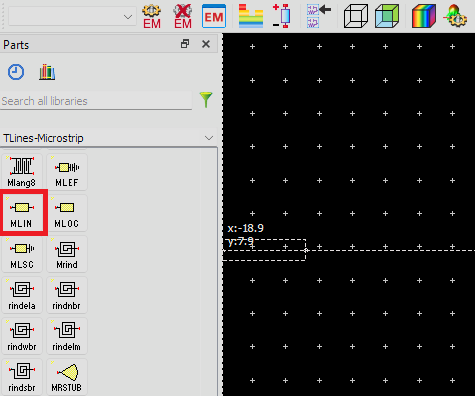
\includegraphics[width=8cm]{figures/metodologia/metologia1.png}
    \caption{Parte utilizada para dibujar las secciones del filtro}
    \label{fig:metologia_mlin}
\end{figure}

Colocar el elemento en el área de trabajo demarcado por la zona oscura. Una vez colocado el elemento, darle doble click izquierdo para abrir el panel de parámetros que se puede observar en la Figura \ref{fig:metologia_mlin_dimensiones}. \\

\begin{figure}[!ht]
    \centering
    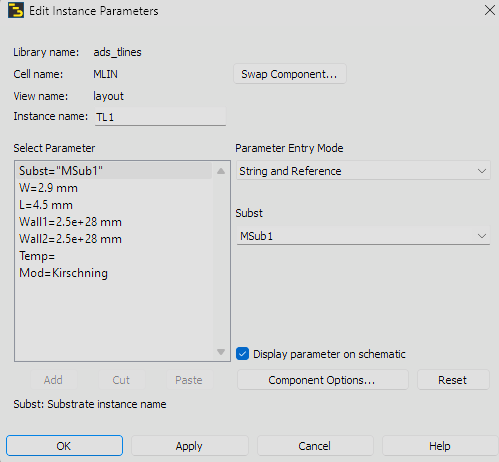
\includegraphics[width=8cm]{figures/metodologia/metologia2.png}
    \caption{Panel de parámetros del elemento \texttt{MLIN}}
    \label{fig:metologia_mlin_dimensiones}
\end{figure}

Con los pasos mencionados anteriormente, inserte las secciones necesarias utilizando los datos mostrados en la tabla \ref{table:metodologia_dimensiones} hasta formar la estructura mostrada en la figura \ref{fig:metologia_secciones_filtro}, donde el ancho corresponde al parámetro \texttt{W} y el largo a \texttt{L}. \\

\begin{table}[!ht]
\centering
\caption{Dimensiones de las secciones del filtro}
\label{table:metodologia_dimensiones}
\begin{tabular}{|c|c|c|}
\hline
Sección & Ancho {[}mm{]} & Largo {[}mm{]} \\ \hline
TL1     & 2.9            & 4.5            \\ \hline
TL2     & 24.7           & 1.68           \\ \hline
TL3     & 0.66           & 10.145         \\ \hline
TL4     & 24.7           & 4.057          \\ \hline
TL5     & 0.66           & 4.202          \\ \hline
TL6     & 2.9            & 4.5            \\ \hline
\end{tabular}
\end{table}

\begin{figure}[!ht]
    \centering
    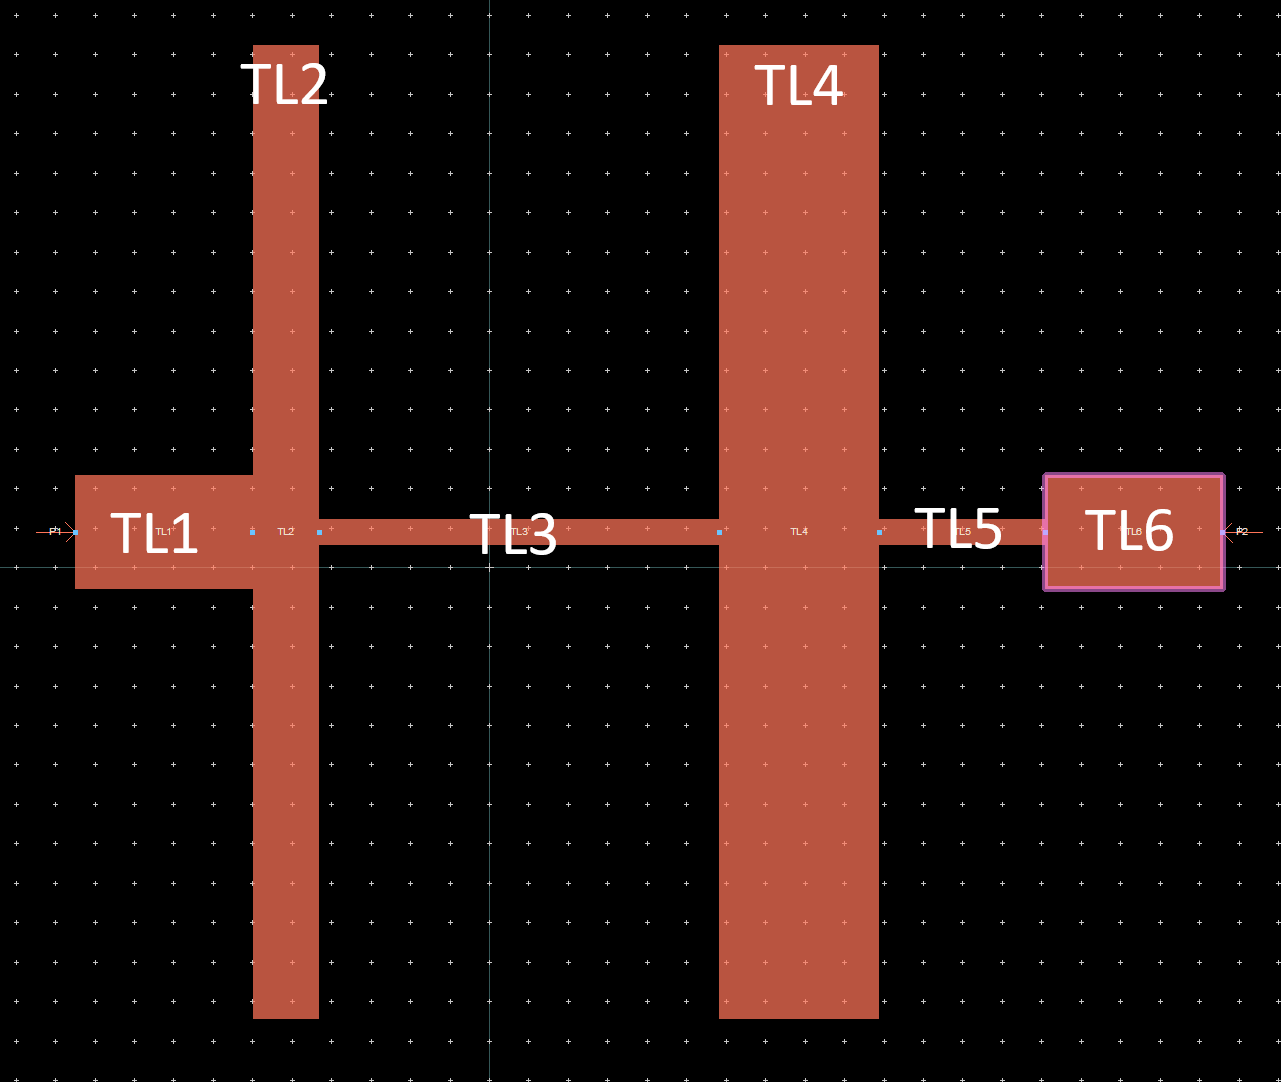
\includegraphics[width=8cm]{figures/metodologia/metologia3.png}
    \caption{Secciones del filtro}
    \label{fig:metologia_secciones_filtro}
\end{figure}

Una vez completada la estructura del filtro, puede proceder a agregar los pines para la simulación \texttt{EM}, para eso haga click en \texttt{Insert} y seleccione la opción \texttt{Pin}. Coloque uno en la conexión restante de \texttt{TL1} y otro en la conexión restante de \texttt{TL6}. \\

\subsection{Creación del substrato}

Crear un nuevo substrato haciendo click derecho sobre la carpeta del proyecto, seleccionar la opción \texttt{New substrate}. \\

Modifique el substrato para que se vea como el mostrado en la figura \ref{fig:metologia_substrato}. La capa del dieléctrico debe tener una constante de permeabilidad de 4.6, una tangente de pérdidas de $0.0023$, y un espesor de 1.6mm. \\
\begin{figure}[!ht]
    \centering
    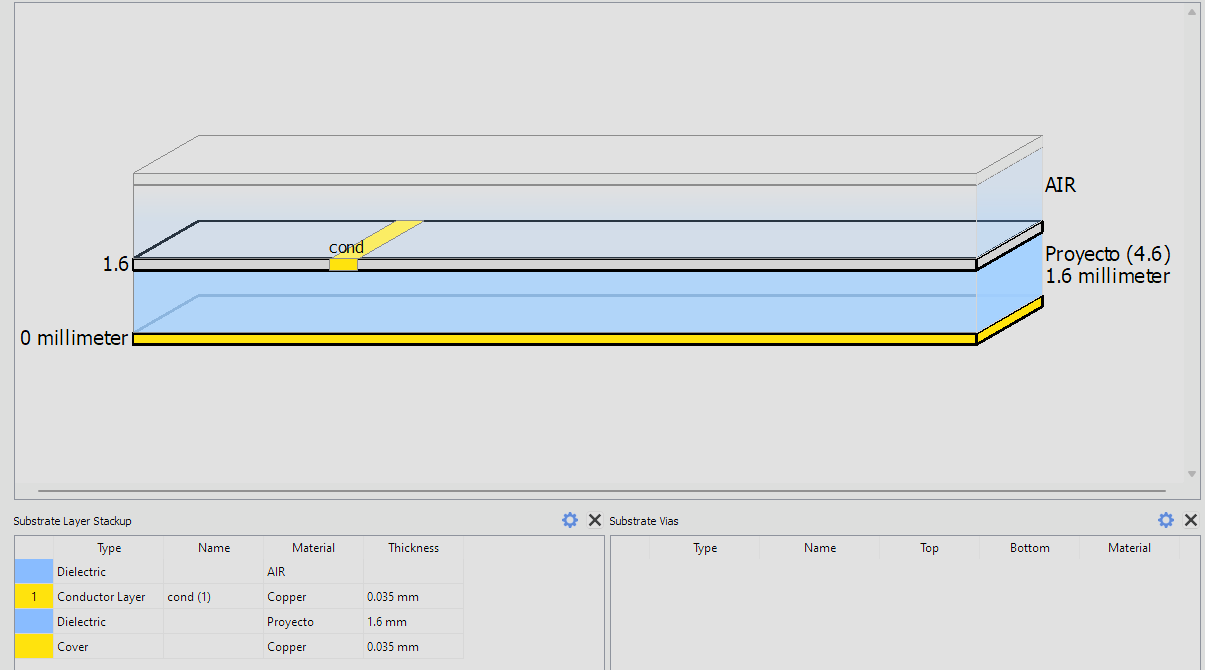
\includegraphics[width=8cm]{figures/metodologia/metologia4.png}
    \caption{Capas del substrato}
    \label{fig:metologia_substrato}
\end{figure}

\subsection{Simulación electromagnética}

Haga click derecho sobre la carpeta que contiene el layout y seleccione la opción \texttt{New} y posteriormente \texttt{EmSetup}. Seleccione con doble click el archivo creado.
En la pestaña de \texttt{Ports} refresque la información utilizando las 2 flechas verdes en la parte superior izquierda de la ventana. Posteriormente, regrese a la pestaña \texttt{FEM} y seleccione el tipo de simulación \texttt{EM Simulation/Model} utilizando el simulador \texttt{FEM}. En la parte inferior derecha selecciona la opción para generar parámetros y presione el botón \texttt{Simulate}.

\section{Resultados}

Utilizando el simulador FEM de ADS se obtuvieron los parámetros \textit{S} del filtro analógico utilizando micro strips. El resultado obtenido se muestra en la figura     \ref{fig:resultado_parametros_s}. Se puede observar que el filtro paso-bajo tiene una frecuencia de corte de -3.5 dB a 1.67 GHz.

\begin{figure}[!ht]
    \centering
    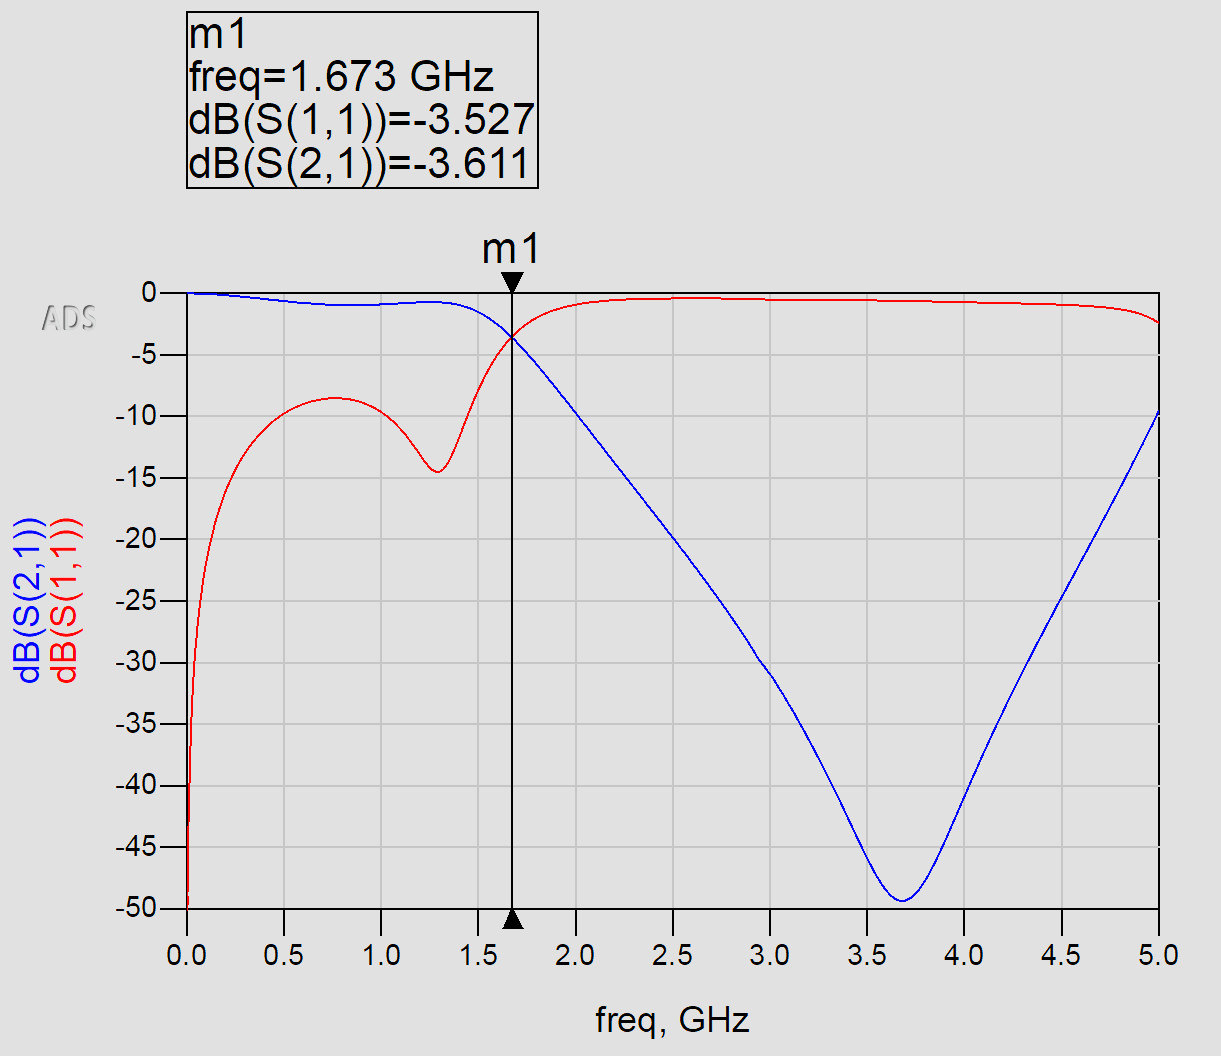
\includegraphics[width=8cm]{figures/resultado.png}
    \caption{Simulación de parámetros S del filtro}
    \label{fig:resultado_parametros_s}
\end{figure}

\section{Discusión}


\section{Conclusiones}

El diseño presentado en el \textit{Advanced Design System-Circuit Design Cookbook 2.0. Keysight Technologies} para un filtro analógico de tipo microstrip posee algunas falencias en su guía, ya que presenta información confusa en algunos casos. Un ejemplo de esto es el grosor del material para el dieléctrico FR4 que en una sección indican que es de 4.6 mm pero en otra imagen muestran un grosor de 1.6 mm, y es este último el valor que provee resultados similares a los adjuntos en el manual. Aún así, esta guía presenta una fascinante técnica para la creación de filtros utilizando microstrips, aprovechando las propiedades de impedancia y geometría para buscar las características deseadas. El propio material identifica que el filtro propuesto no cumple con la frecuencia de corte deseada, y proveen una solución útil y enseñan los pasos para realizar un barrido para la optimización del filtro, lo cual expande las oportunidades de diseño que tienen los ingenieros en electrónica para buscar soluciones ópticas que satisfagan los requerimientos del sistema.

\section*{References}
\bibliographystyle{IEEEtran, bibliography/bibliography.bib}

\end{document}
